Following the taxonomy of \cite{kritzinger2018digital}, the proposed framework operates as a digital shadow rather than a fully bidirectional digital twin. Information flows from the physical project to the probabilistic digital representation through structured data uploads compiled by site engineers, while decisions derived from the model outputs remain mediated by human agents. This positioning reflects the operational reality of construction projects, where automated actuation on the physical system is precluded by contractual, regulatory, and human judgment constraints.

The framework is implemented in Python and exposed through a client and server architecture. A Streamlit based web interface \citep{streamlit} handles data ingestion and visualization, while the inference engine runs on the server side. Monte Carlo sampling of activity durations relies on the \texttt{Scipy}, which natively supports the triangular distributions adopted in this work, and Bayesian inference is performed with the library \texttt{pgmpy}. Activity durations are sampled with $N = 10,000$ realizations, a value consistent with the Monte Carlo sample sizes.% commonly adopted in stochastic CPM analysis [citar 1 ou 2 trabalhos]. 

The Bayesian network is constructed directly from the CPM precedence graph: each activity is mapped to a node, arcs follow the precedence relations, and conditional probability tables are estimated from the empirical relative frequencies of the sampled durations after discretization. The discretization resolution is a user defined parameter; integer days are adopted as the default because they match the operational granularity at which construction schedules are managed and reported, ensuring that each discrete state in the Bayesian network corresponds to an observation directly realizable in the field. 

The framework takes as input a simple activity table containing, for each activity, its identifier, predecessors, and the minimum, mode, and maximum duration values that parameterize the triangular distribution. A public web deployment of the tool is available at \url{https://civilprobabilisticplanning.streamlit.app}, where readers can reproduce the analyses presented in Section 5 and apply the framework to their own planning scenarios.

The digital twin assessment pipeline is divided into 3 categories or activities: (\textit{a}) uploading the desired scenario, (\textit{b}) choosing the adopted risk level, and (\textit{c}) applying the evidence concept and its propagation in the complex network. Each of these items is detailed to provide an overview of how the digital twin supports the desired planning analysis.

% \subsubsection{Dataset Upload and Critical Path Method Scenarios}

% The desired scenario dataset is transferred via a Streamlit file-upload component configured to accept only the \textit{xlsx} Excel format. Other formats are easy to implement. The file should contain a tab with the following columns properly filled in: (a) Code, (b) Task Name, (c) Predecessors, (d) Min., (e) Mode, (f) Max., and each row represents an activity in the plan. A scenario template is available in the application for download and editing to suit the user's plan.

% The ``\textit{Code}'' column contains the unique identifier for each activity. If the same identifier is present in more than one activity, the system will return an error as the application cannot perform the analyses correctly.

% The column ``\textit{Task Name}'' stores the name of the activity, which will be used as a visual identifier for the user during analysis. Therefore, we recommend that it also be represented by a unique value.

% The ``\textit{Predecessors}'' column indicates the code of the preceding activity. In the cases where there is more than one preceding activity, they must be separated by a comma. For the first activity in the scenario, this column should be filled with ``-''. The system supports only one initial activity, and the user must account for this when entering scenarios.

% Before running the application, the user must initially determine the duration (in days) of each activity and fill in the ``Min.'' column with the estimated minimum duration, the ``Mode'' column with the most likely duration (mode), and the ``Max.'' column with the maximum duration the activity can have.

% After data input, the simulator performs a probabilistic time analysis of all planning activities and ultimately returns a sample of 10,000 scenarios from the set of activities, regardless of their size. The sample size can be changed. However, in the initial versions of the software, this value was standardised. For scenario analysis and generation, we use the \textit{parepy-toolbox} library, which supports triangular distributions; therefore, the minimum, mode, and maximum durations of each activity must be specified. Figure \ref{fig:hist_active_1} shows the histogram of the sample distribution of a given activity with minimum, mode, and maximum values equal to 2.0, 3.0 and 6.0, respectively.

% \begin{figure}
%     \centering
% 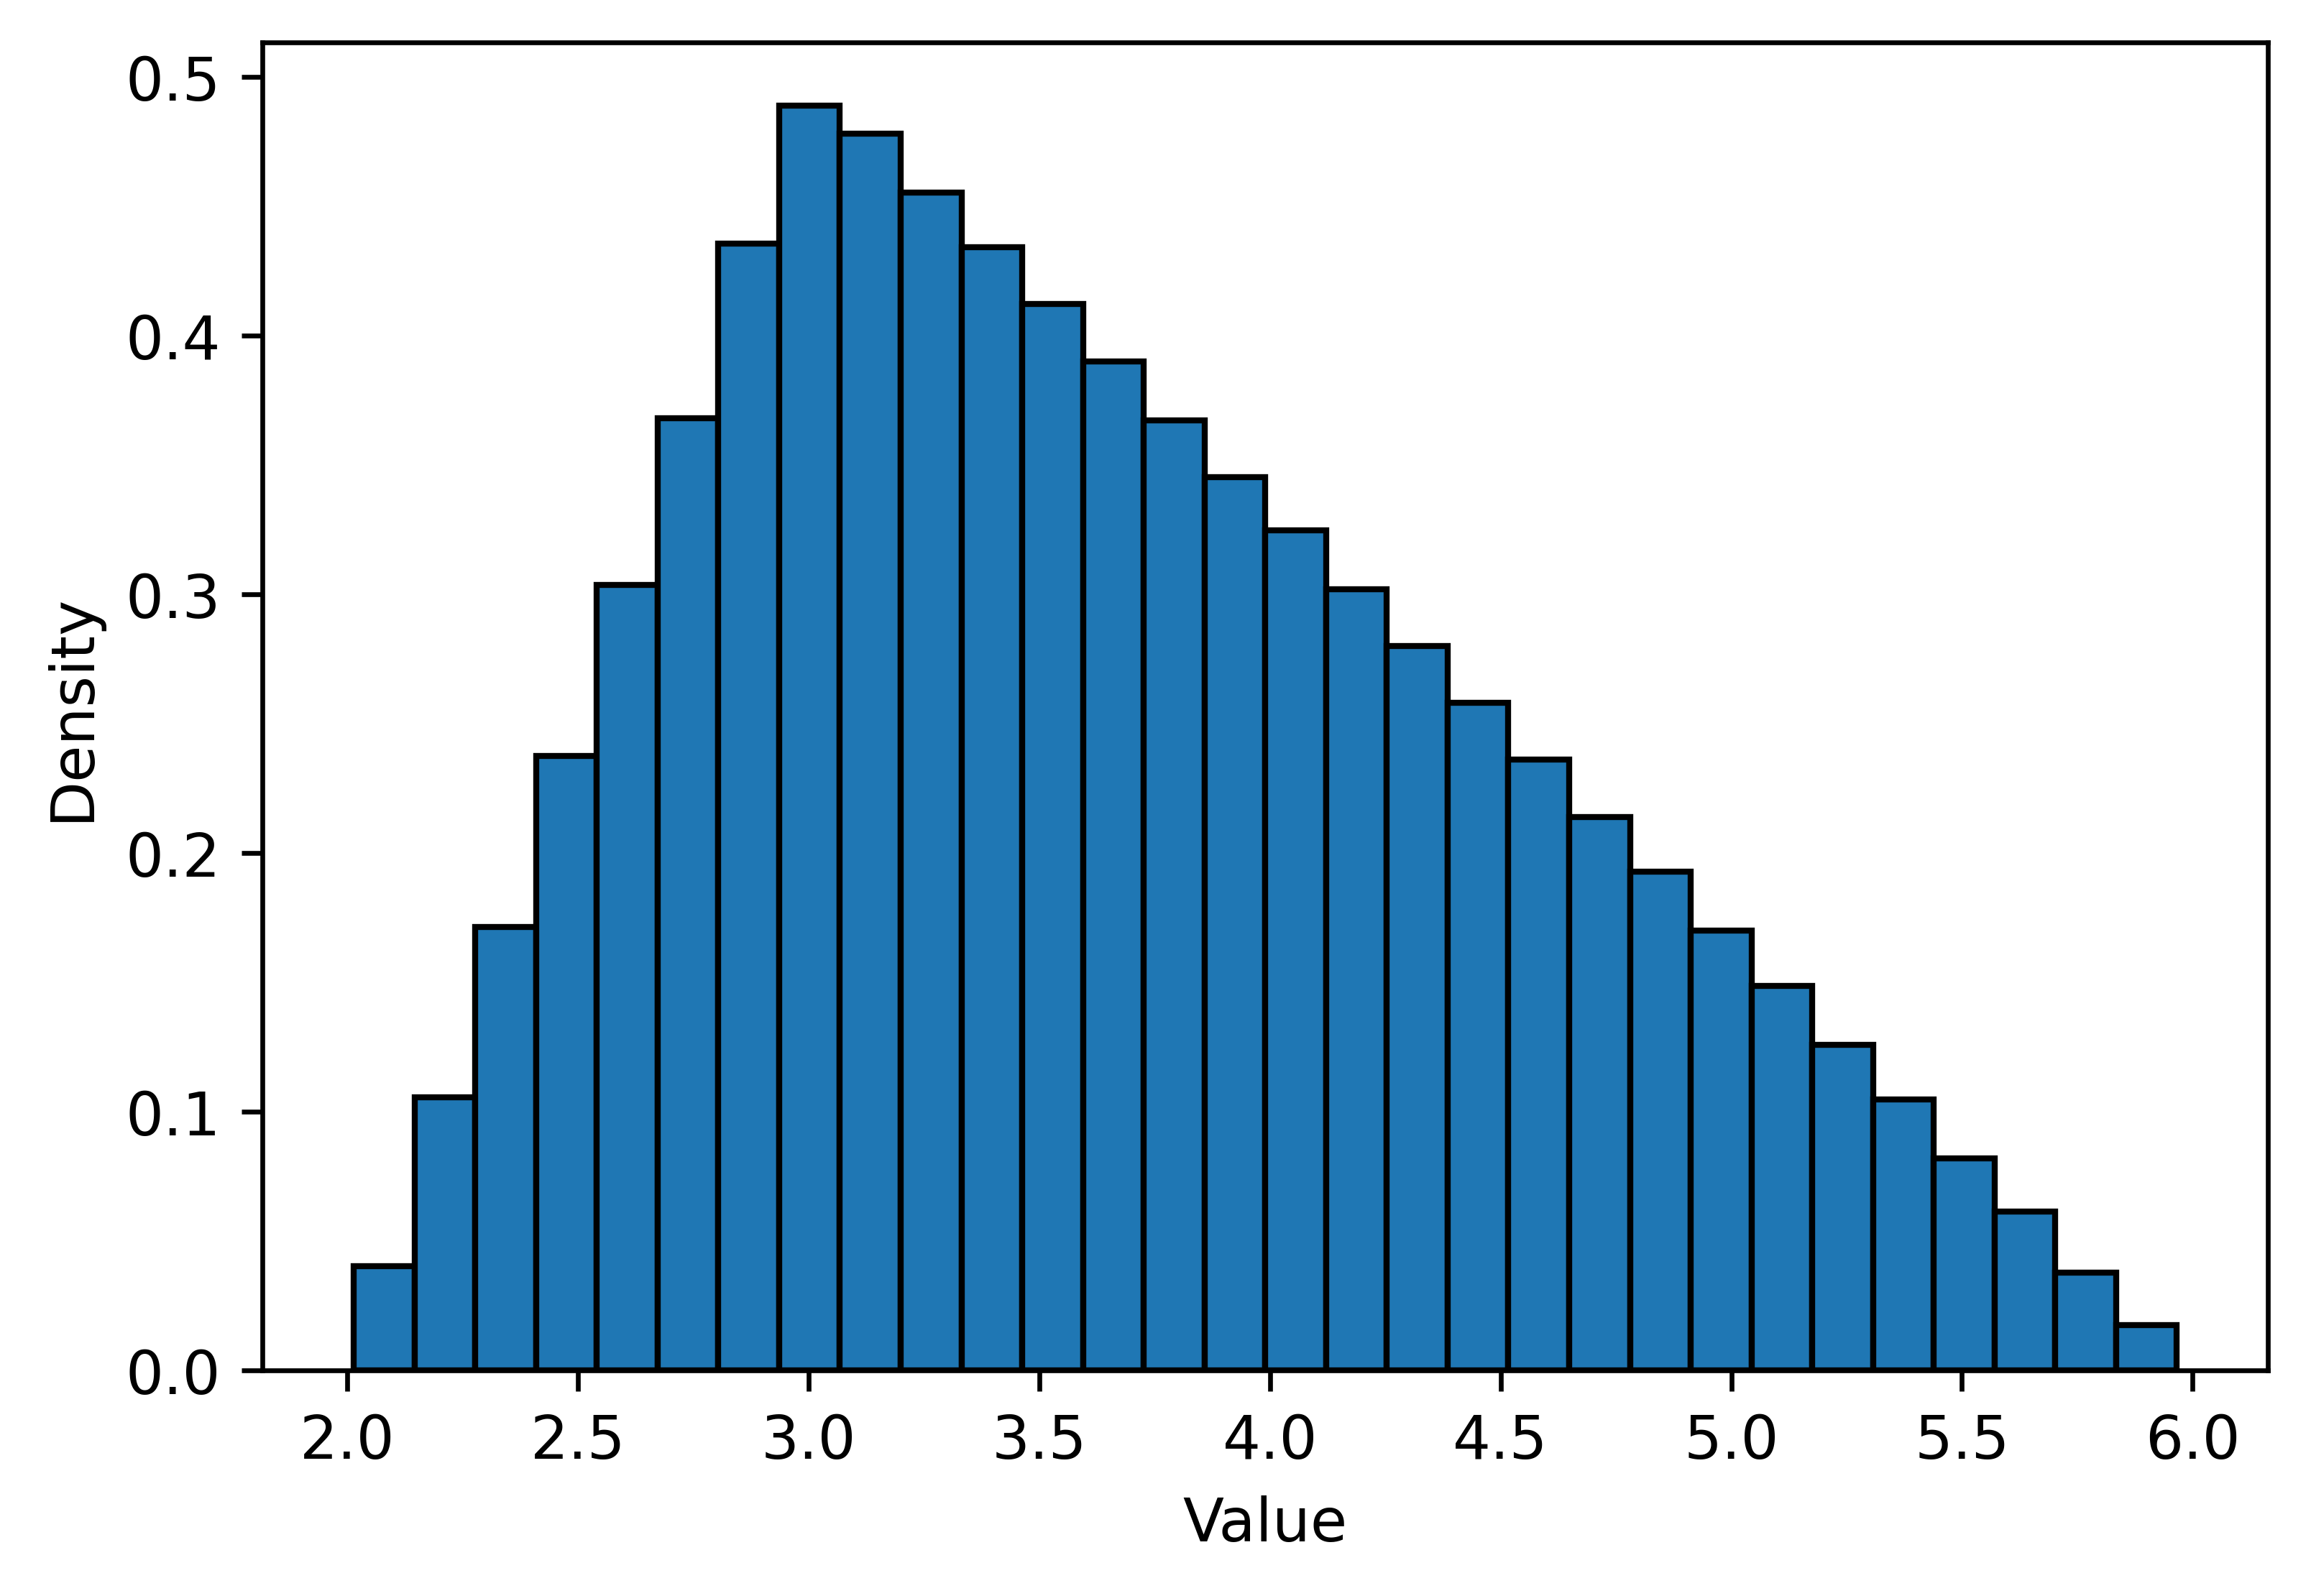
\includegraphics[width=0.6\linewidth]{images/fig_hist_active_1.png}
%     %\caption{Grafo do Plano  do projeto.}
%     \caption{Illustration of the histogram of an activity}
%     \label{fig:hist_active_1}
% \end{figure}


% \subsubsection{Risk analysis}

% Once the scenario database is built, the application provides functionality to perform risk analysis for the duration of the planning horizon; these concepts were explained in section \ref{sub:var}. To perform the risk analysis, the user must specify the desired confidence level, which must be between 0 and 1. The application will then display the VaR and CVaR for that planning horizon in days, based on the provided confidence level.

% \subsubsection{Belief propagation}

% The Bayesian Network is trained using Conditional Probability Tables (CPTs) derived from the scenario database. To compute the CPTs, data from all scenarios are first grouped by activity. The corresponding duration values are then rounded and discretized to identify a finite set of distinct states. Subsequently, the probability associated with each state is estimated from its empirical relative frequency, computed as the ratio between the number of occurrences of the state and the total number of observations in the dataset, as described in Algorithm~\ref{alg:discretization_integer_days}. Table~\ref{tab:cpt_example} presents an example of a resulting CPT obtained from the activity duration distribution illustrated in Figure~\ref{fig:hist_active_1}.

% \begin{algorithm}[H]
% \caption{Discretization by Integer Days}
% \label{alg:discretization_integer_days}
% \begin{algorithmic}[1]
% \REQUIRE $DF$ — matrix of continuous samples
% \ENSURE $\Theta$ — discretization parameters

% \STATE $DF^{*} \leftarrow \mathrm{round}(DF)$
% \STATE $\Theta \leftarrow \emptyset$

% \FOR{each activity $a$ in $DF^{*}$}
%     \STATE Compute relative frequencies of values in column $a$
%     \STATE $S_a \leftarrow$ sorted set of observed integer values
%     \STATE $P(s) \leftarrow$ empirical probability of each $s \in S_a$
%     \STATE Define value mapping $f_a(s) = s$
%     \STATE $\Theta[a] \leftarrow \{S_a, f_a, P(s)\}$
% \ENDFOR

% \RETURN $\Theta$
% \end{algorithmic}
% \end{algorithm}


% \begin{table}[h]
% \centering

% \caption{CPT of an activity}
% \begin{tabular}{cc}
% \toprule
% State & Probability \\
% \midrule
%  2 & 0.0625 \\
%  3 & 0.4167 \\
%  4 & 0.3333 \\
%  5 & 0.1667 \\
%  6 & 0.0208 \\
% \bottomrule
% \label{tab:cpt_example}
% \end{tabular}
% \end{table}

% Once the network is trained, the system allows the user to make inferences as the scheduled activities are completed. This enables updating the total project duration estimate based on observed performance. It is important to note that the values available for adding evidence are limited to the states defined in the CPT. Therefore, if an activity is completed with a duration outside the range (minimum and maximum) contained in the original dataset, the model will not allow the assignment of that specific value.

% After processing the inferences, the application generates an updated conditional probability distribution and presents the new project completion metrics. The system visually highlights the minimum and maximum duration scenarios, as well as the most likely value (mode of the distribution), allowing a clear view of the residual uncertainty in planning.

\subsection{Toy problem}
To illustrate the application of the digital model, a civil construction schedule is presented in Table \ref{tab:toyproblem}. This dataset represents a simplified planning scenario structured as a toy problem for methodological demonstration. The tasks follow well-defined precedence relationships, and their durations are specified using minimum, most likely, and maximum estimates, enabling controlled experimentation and comparative analysis within the proposed framework.

\begin{table}[htpb!]
    \centering
    \caption{Toy problem: civil construction schedule used to exemplify the application of the digital model, including task precedence relationships and minimum, most-likely, and maximum duration estimates.}
    \label{tab:toyproblem}
    \begin{tabular}{|l|l|l|l|l|l|}
    \hline
        \textbf{Code} & \textbf{Task Name} & \textbf{Predecessors} & \textbf{Min.} & \textbf{Mode} & \textbf{Max.} \\ \hline
        A & Activity 1 & -  & 0.5 & 1.0 & 2.0 \\ \hline
        B & Activity 2 & A  & 2.0 & 3.0 & 4.0 \\ \hline
        C & Activity 3 & A  & 0.5 & 1.0 & 1.5 \\ \hline
        D & Activity 4 & B  & 3.0 & 4.0 & 5.0 \\ \hline
        E & Activity 5 & C  & 2.0 & 3.0 & 6.0 \\ \hline
        F & Activity 6 & D,E & 1.8 & 2.0 & 4.0 \\ \hline
    \end{tabular}
\end{table}

\subsubsection{Scenarios}
%Mostra que a plataforma amostra cenários estatisticos do problema qie v quer analisar

%Com a inserção do dataset na plataforma, a mesma realiza a amostragem de 10000 cenários e disponibiliza da descrição estatística do novo dataset de amostras gerado conforme a figura \ref{fig:df_scenarios}.

Once the dataset is loaded onto the platform, it samples $10,000$ scenarios and provides a statistical description of the resulting sample. Figure \ref{fig:df_scenarios} shows the output of our system with the descriptive statistics for each task.



\begin{figure}
    \centering
    \fbox{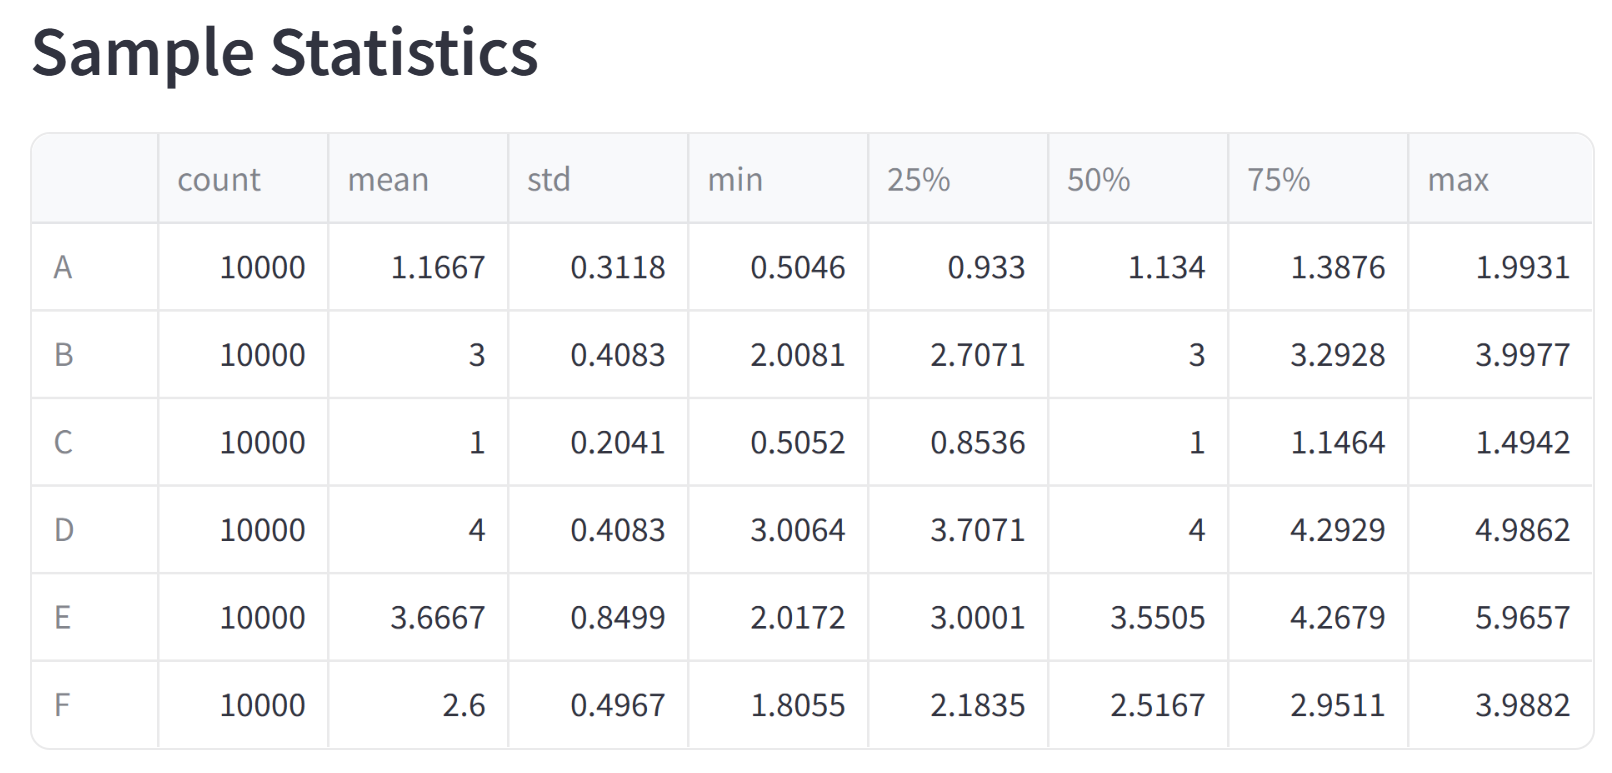
\includegraphics[width=1\linewidth]{images/sample_statistics.png}}
    \caption{System illustration: Description of the dataset containing all scenarios generated in the sampling.}
    \label{fig:df_scenarios}
\end{figure}

\subsubsection{Graph analysis and Critical Path}
%Mostra quais as capacidades do modelo em gerar cenários de caminho critico
%É possível fazer uma análise do grafo do dataset, definindo qual o ponto de início e o ponto de fim do caminho crítico, conforme a figura \ref{fig:graph_analysis}

We perform a graph analysis of the dataset, defining the starting point (activity 1) and ending point (activity 6) of the critical path, as shown in Figure \ref{fig:graph_analysis}.

\begin{figure}
    \centering
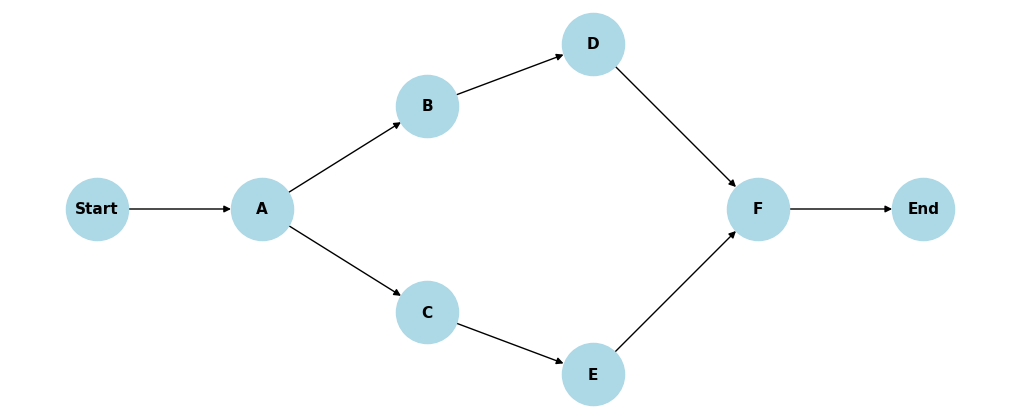
\includegraphics[width=0.6\linewidth]{images/fig2_grafo_direcionado.png}
    %\caption{Grafo do Plano  do projeto.}
    \caption{Graph of the project plan.}
    \label{fig2:031024}
\end{figure}

Figure \ref{fig:graph_analysis} illustrates the input interface of our system.

\begin{figure}
    \centering
    \fbox{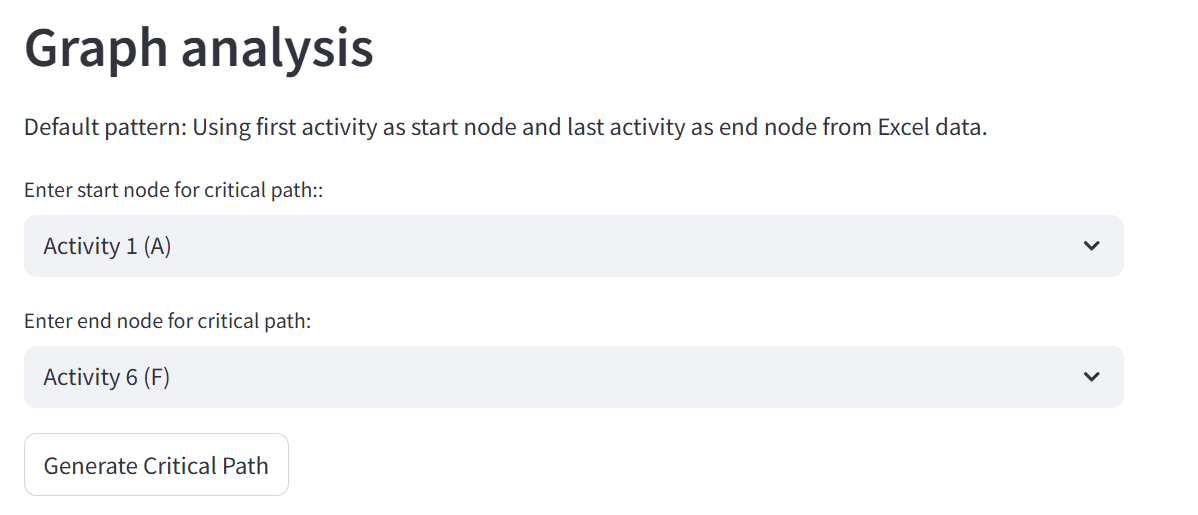
\includegraphics[width=1\linewidth]{images/define_path.png}}
    %\caption{Inputs para definir nó de início e nó de fim}
     \caption{System illustration: Inputs to define start node and end node.}
    \label{fig:graph_analysis}\end{figure}

%Para cada cenário gerado na amostragem, o sistema gera um grafo e o seu respectivo caminho crítico, ao fim disso é gerado um gráfico de densidade do tempo total daquele caminho crítico conforme a figura \ref{fig:makespan_scenarios}. Nesse gráfico é possivel observar que, para esse exemplo, grande parte dos cenários mostram que o planejamento irá durar 11 dias.

%HK. Acho quee a Figura 6 nao eh densidade. Eh um histograma (contendo a frequencia do tempo total). Funcao densidade de probabilidade eh mais usada para distribuicoes continuas. No caso, nao eh uma distribuicao de probabilidades, mas eh um histograma com a frequencia (observada)
For each scenario generated in the sampling, the system builds a graph and its respective critical path. The system also creates a histogram of the total time of that critical path, that could be a proxy of a probability distribution of the project makespan, as shown in figure \ref{fig:makespan_scenarios}.

The statistical descriptive analysis of the total project duration is summarized in Table \ref{tab:descriptive_stats}. The expected project makespan (mean) is 10.77 days, with a median of 10.75 days and a standard deviation of 0.82 days. The results range from a minimum of 8.10 days to a maximum of 13.90 days. Within this framework, we can identify that the most probable scenario (mode) is approximately 11 days.

\begin{table}[h]
\centering
\caption{Descriptive statistics of the project makespan (10,000 scenarios).}
\label{tab:descriptive_stats}
\begin{tabular}{l|r}
\hline
\textbf{Statistic} & \textbf{Value (Days)} \\ \hline
Sample Count & 10,000 \\
Mean & 10.77 \\
Standard Deviation & 0.82 \\
Minimum & 8.10 \\
First Quartile (25\%) & 10.20 \\
Median (50\%) & 10.75 \\
Third Quartile (75\%) & 11.32 \\
Maximum & 13.90 \\ \hline
\end{tabular}
\end{table}

%Within this framework, we can identify that the most probably scenario is that the planning will last 11 days. Other metrics can also be calculated. \textcolor{red}{Complementar For instance, the expected project makespan is XXXX (incluir o valor médio) and the standard deviation XXX (incluir o desvio-padrao). Talvez adcionar as principais estatisticas descritivas (minimo, media, mediana, maximo, desvio-padrao) da tarefa completa. Padronizar as tabelas e figuras (para nao ficar em formatos ou tamanhos ou fontes muito diferentes)}.

\begin{figure}
    \centering
    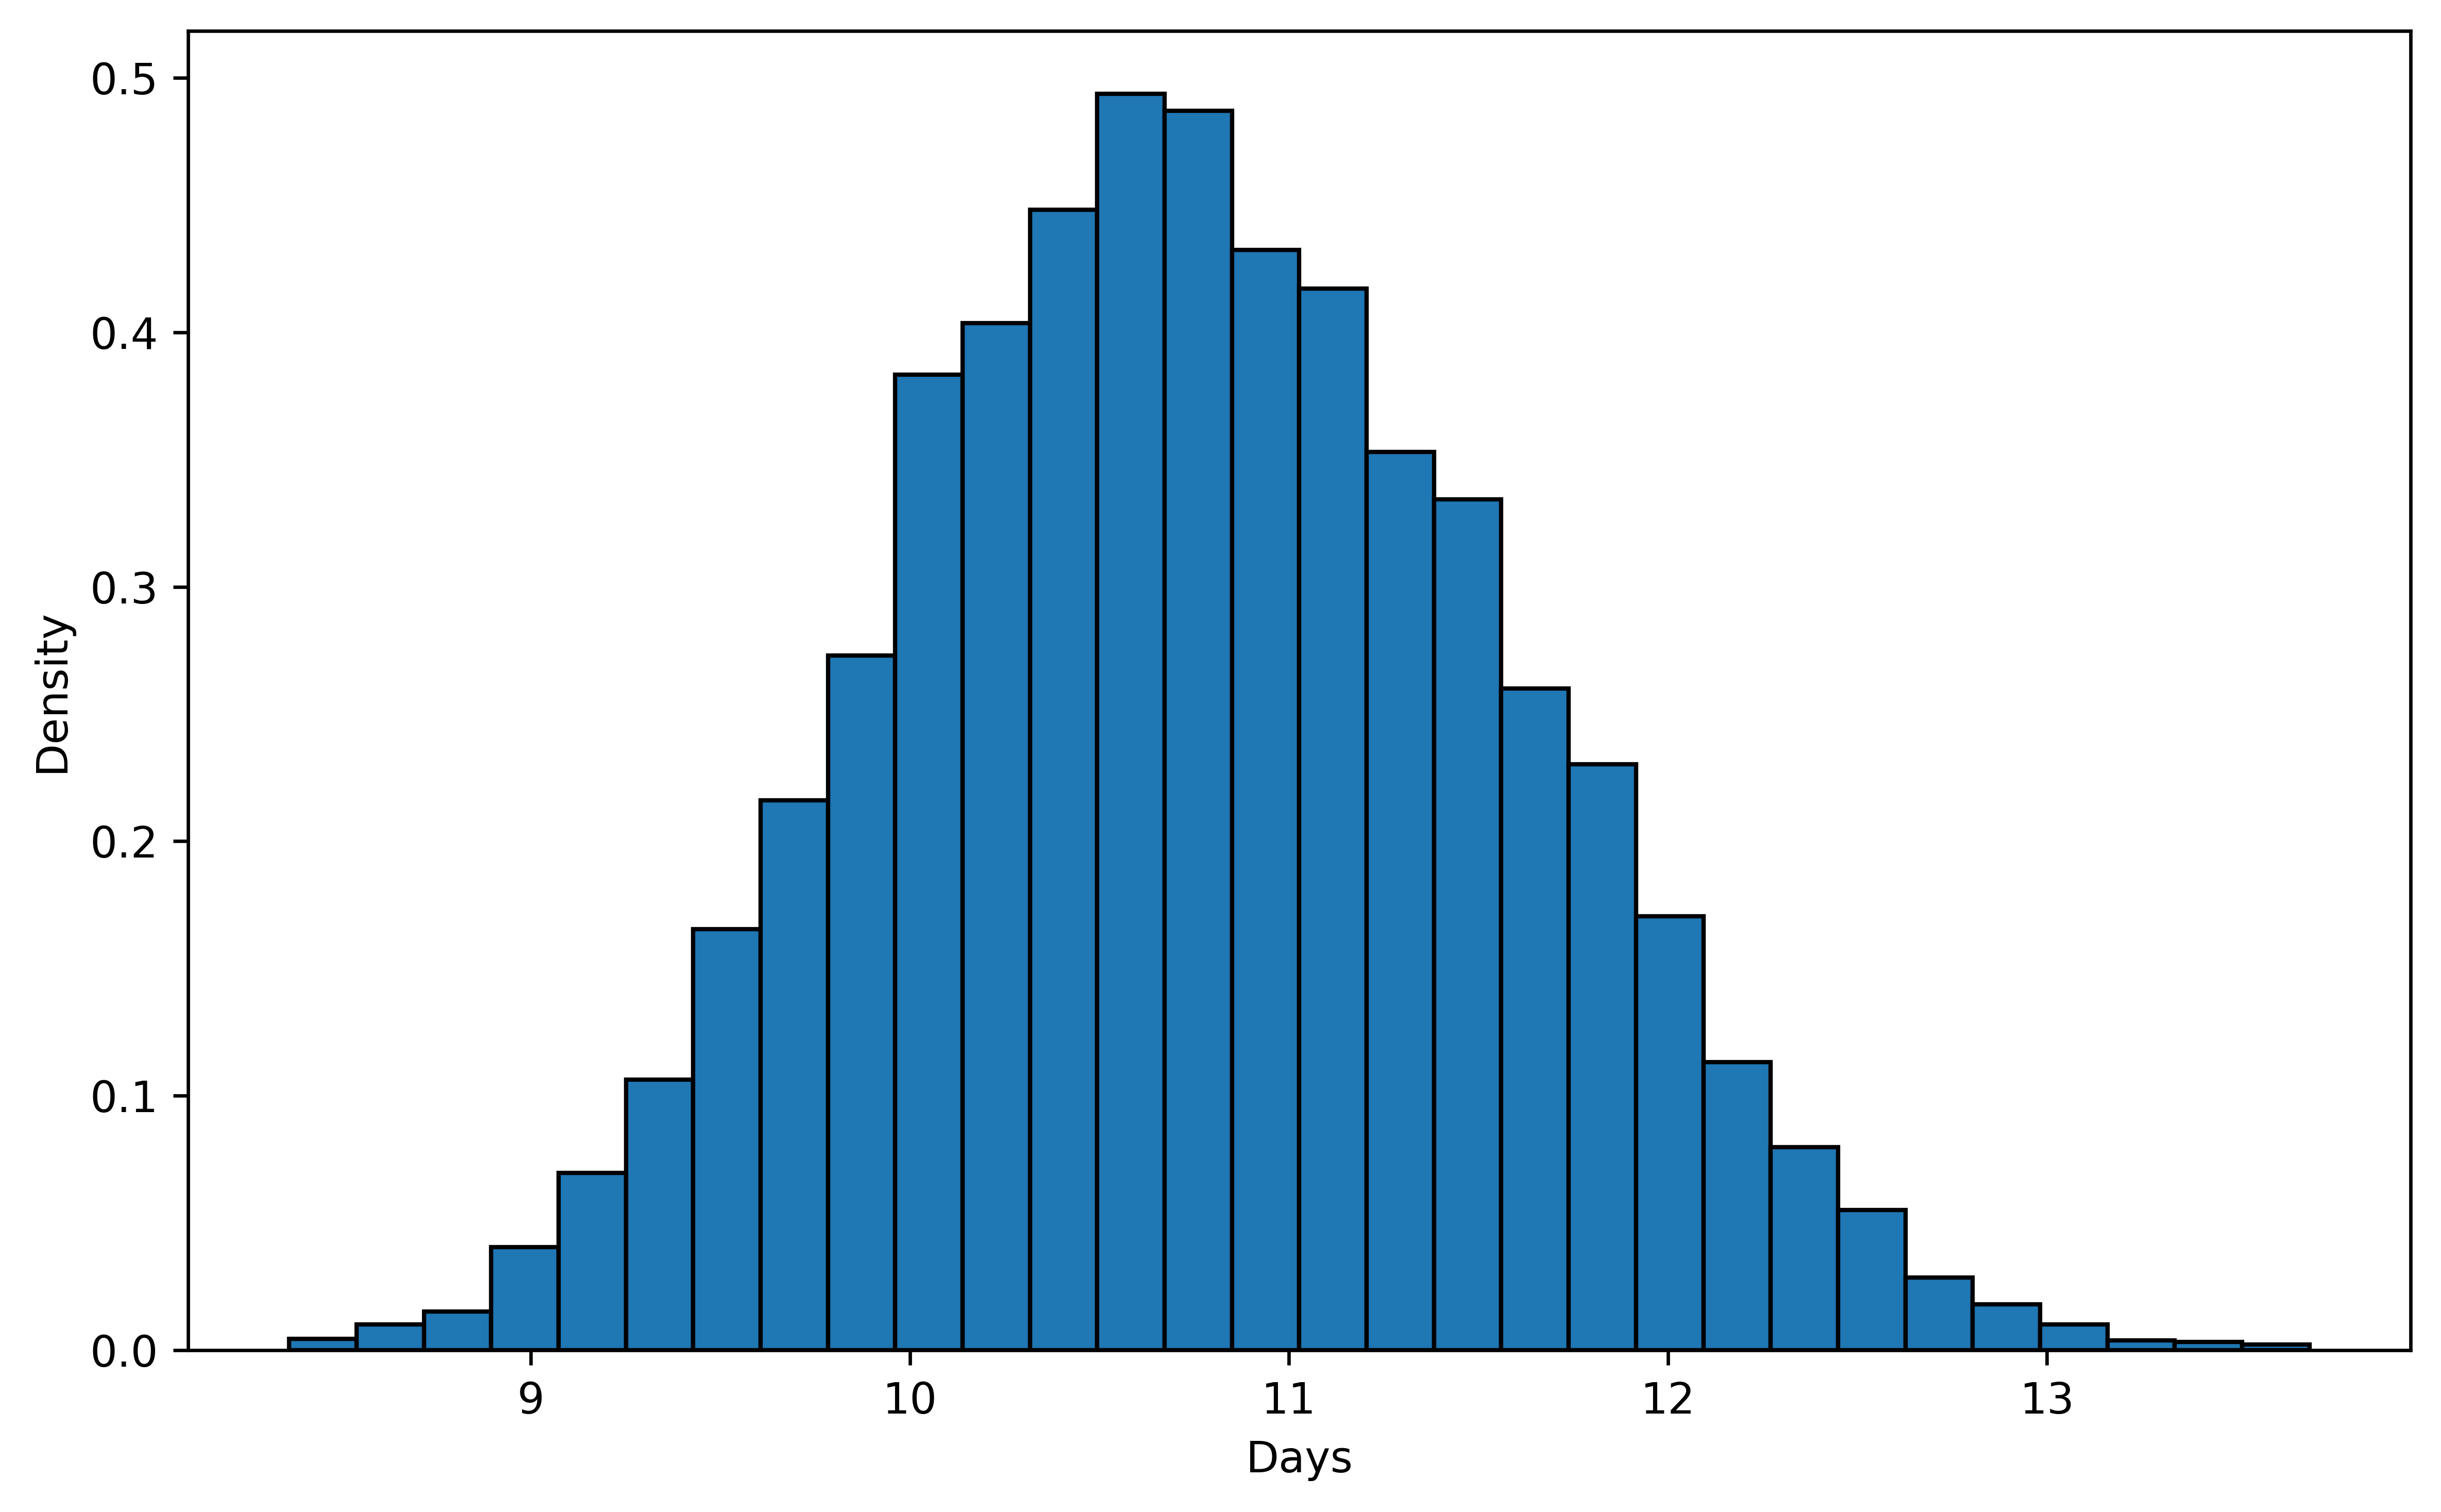
\includegraphics[width=1\linewidth]{images/makespan_distribution.png}
    \caption{Makespan distribution}
    \label{fig:makespan_scenarios}
\end{figure}

\subsubsection{Risk analysis}
%Mostra que ele faz uma análise de risco em função de um alpha declarado
%Dados os caminhos críticos calculados é possível fazer uma análise de risco, onde é possível definir com um certo indice de confiança, qual será o tempo máximo de duração do planejamento, e caso venha a ultrapassar esse valor, qual será o valor médio que pode durar. Para o calcúlo basta inserir o indice de confiança no input, conforme a figura \ref{fig:risk_analysis}. Nessa figura é mostrado que para um índice de confiança de 0.95, que o Var é de cerca de 12.20 dias e o CVar é de 12.53 dias. Para o caso onde o índice de confiança é de 0.8 o Var cai para 11.48 dias e o Cvar para 11.95, e caso o índice seja 0.5 o Var será 10.75 dias e o Cvar 11.43 dias. Isso mostra que esse tipo de problema, quanto menor o índice de confiança esperado, menor será o valor

Given the simulated critical paths, we can perform a thorough risk analysis. For instance, we can define, with a certain confidence level, the maximum duration of the planning, and if it exceeds that value, what the average duration could be. To calculate these statistics, we simply enter the confidence level as an input in the system, as depicted in figure \ref{fig:risk_analysis}. This figure shows that, for a confidence level of 0.95, i.e., $\alpha = 5\%$ the $VaR_{5\%}$ is approximately 12.20 days and the $CVaR_{5\%}$ is 12.53 days. Therefore, the results show that, for this toy exercise, the critical path will not last more than the 12.20 days, with a 95\% confidence. There is only a 5\% probability of the project makespan exceeding the $VaR$ 12.20 days. In the scenarios that the project makespan lasts more than 12.20 days, the average of the duration of the project will be $CVaR$ of 12.53 days. 

Given that the simulated scenarios allow building a probability distribution, results for other confidence levels can also be calculated, leading to a more thorough analysis of the risk of the makespan. For example, using a confidence level of 0.8, the $CVaR_{20\%}$ drops to 11.48 days and the $CVaR_{20\%}$ to 11.95 days. and if the confidence level is 0.5, the $VaR_{50\%}$ is 10.75 days and the $CVaR_{50\%}$ 11.43 days. %This shows that for this type of problem, the lower the expected confidence level, the lower the value will be.

%\begin{figure}
%    \centering
%    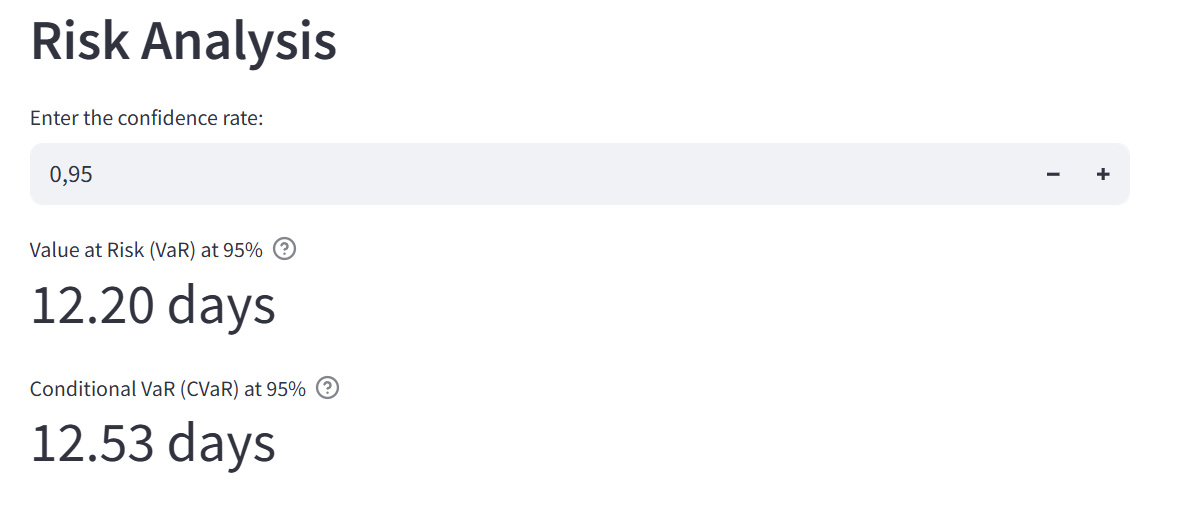
\includegraphics[width=1\linewidth]{images/risk_analysis.png}
%    %\caption{Calculo da análise de risco realizado}
%    \caption{Risk analysis}
%    \label{fig:risk_analysis}
%\end{figure}

\subsubsection{Belief updating}
%Mostra como a propação de evidência é feita no projeto

%Por fim, o sistema treina uma rede Bayesiana usando a CPT dos dados, tendo esse modelo treinado é possível fazer inferências no sistema para recalcular qual será o possível tempo total para a conclusão do projeto, na figura \ref{fig:inference} é possível ver um exemplo de inferência, onde foi informado que a atividade 1 durou extamente 2 dias, com isso, é possível ver qual será a nova previsão em dias para concluir todo o projeto na figura \ref{fig:inferece-result}.

% Finally, the system trains a Bayesian network using the CPT of the data. With this trained model, it is possible to make inferences in the system to recalculate the possible total time for the project completion. Figure \ref{fig:inference} shows an example of this inference, where it was reported that activity 1 lasted exactly 2 days. Therefore, it is possible to see the new prediction in days to complete the entire project in Figure \ref{fig:inference-result}, given the information from activity 1.


%Para demonstração da propoagração de evidências 3 cenários foram estabelecidos e verificados para a determinação da probilidade de duração da atividade final. Os cenários (a) atvidade A com 1 dia e as outros obtidas pro meios de propgarção na rede, (b) Cenários atividade A com 3 dias e atividade B com 4 dias e as outras atividades por meio da rede.


%No cenário A é possível perveber que a quando a atividade A demora 1 dia o cenário mais provável de finalização do empreendimento é de xx dias com probailidade de 0.38. 

%\textcolor{red}{Aprimorar a discussao, indicando a utilidade. In the scenario A, we can identify that, when activity A lasts 1 day, the project is more likely to be completed in XX with a 0.38 probability.}

 
Finally, the system trains a Bayesian network using the CPT derived from the data. With this trained model, it is possible to perform inferences to recalculate the total time for project completion based on real-time updates. Figure \ref{fig:inference} illustrates the interface used for this process, where an evidence was reported: activity 1 lasted exactly 2 days. Figure \ref{fig:inference}.

\begin{figure}[h]
    \centering
    \fbox{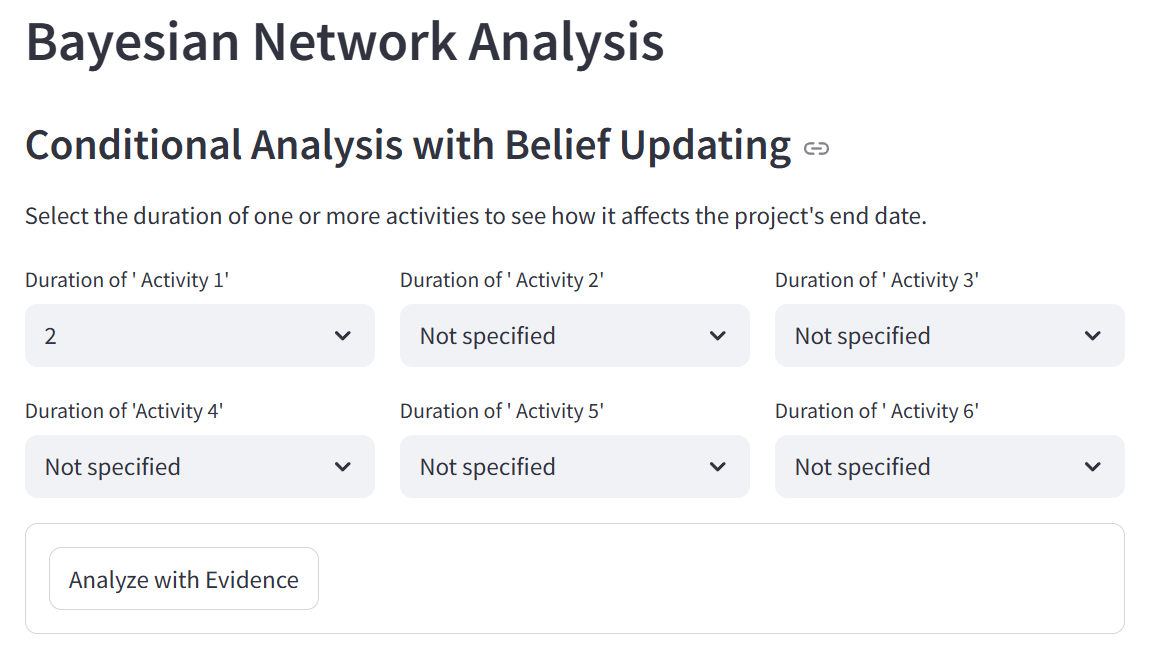
\includegraphics[width=0.8\linewidth]{images/inference.png}}
    \caption{System illustration: Interface for evidence input in the Bayesian Network, showing the selection of observed duration for Activity 1.}
    \label{fig:inference}
\end{figure}

Consequently, the updated prediction for the project makespan is presented in Figure \ref{fig:inference-result}. For this specific inference, the statistical analysis reveals an expected project makespan (mean) of 10.77 days, with a median of 10.75 days and a standard deviation of 0.82 days. The simulated scenarios for this condition range from a minimum of 8 days to a maximum of 14 days, with the most probable completion time occurring at 10 days, presenting a probability of 0.38.

To demonstrate the propagation of evidence, two additional scenarios were established to determine the probability of the final project duration: (a) activity A lasting 1 day, and (b) activity A lasting 3 days combined with activity B lasting 4 days.

\begin{figure}[h]
    \centering
    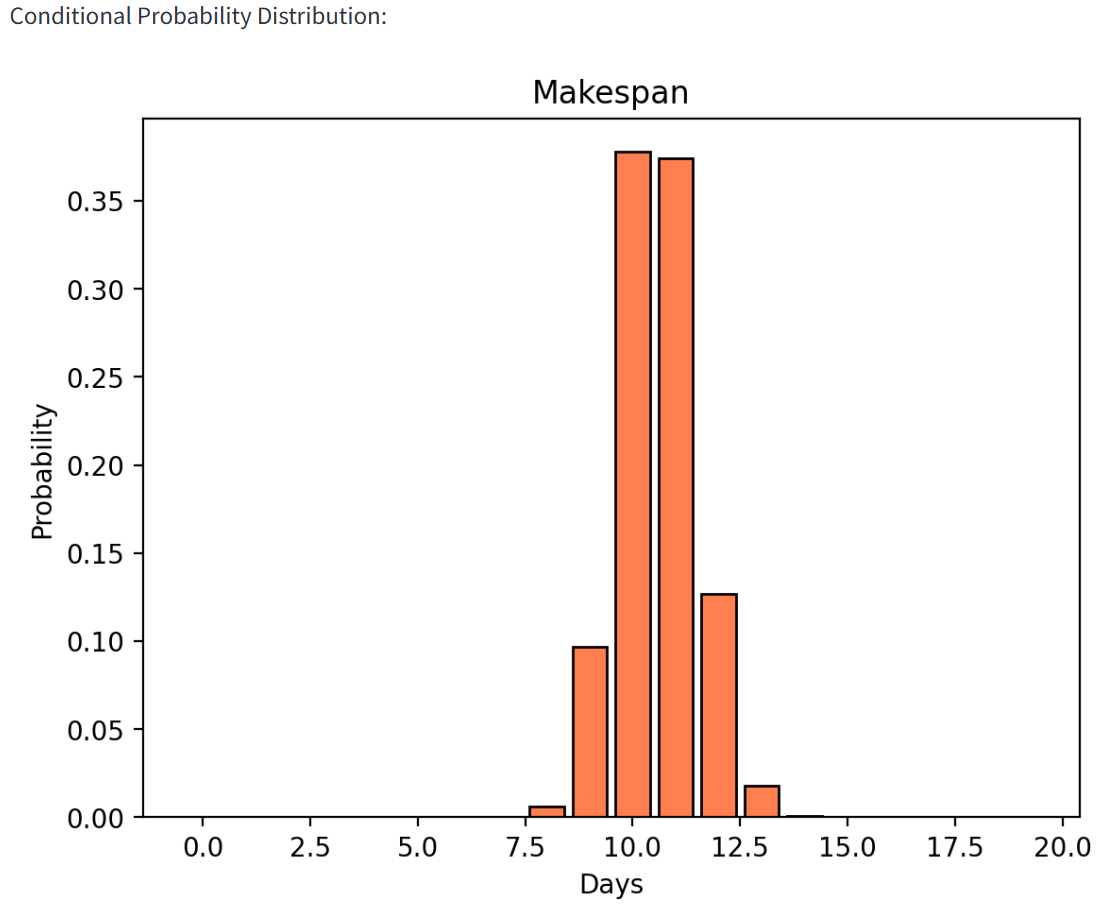
\includegraphics[width=0.8\linewidth]{images/inference_result.png}
    \caption{Probability distribution of the project makespan (Conditional PMF) after evidence propagation for different scenarios.}
    \label{fig:inference-result}
\end{figure}

The results demonstrate the model's utility for dynamic risk management. In Scenario A, when activity A lasts 1 day, the project is most likely to be completed in 9 days ($p=0.38$), within a window of 7 to 13 days. In contrast, Scenario B (Activity A=3 and B=4) shifts the distribution towards a longer duration, where the most probable outcome is 11 days ($p=0.42$), with a tighter range starting at 10 days and reaching a maximum of 14 days. This comparative analysis highlights how the Bayesian approach allows managers to quantify the impact of early task variations on the final deadline, providing a probabilistic confidence interval that is more robust than traditional deterministic methods.